\documentclass{article}
\usepackage[utf8]{inputenc}
\usepackage{a4wide}


%% Copy the following definitions into your preamble. Then copy the
%% tikz figures into your main document and replace "0" in the calls
%% to \shortedgelabel with the correct values. You can highlight edges
%% by adding "draw=red" to their parameters.


\usepackage{tikz}
\usetikzlibrary{matrix,calc,positioning,patterns}
\usetikzlibrary{arrows,automata}

\tikzstyle{horizontal states}=[
    ->,>=stealth',auto,node distance=0.5em and 5em,
    every state/.style={
        minimum size=12mm,
}]
\newcommand{\shortedgelabel}[2]{\ensuremath{#1[#2]}}


\begin{document}
    \begin{center}
    \small
        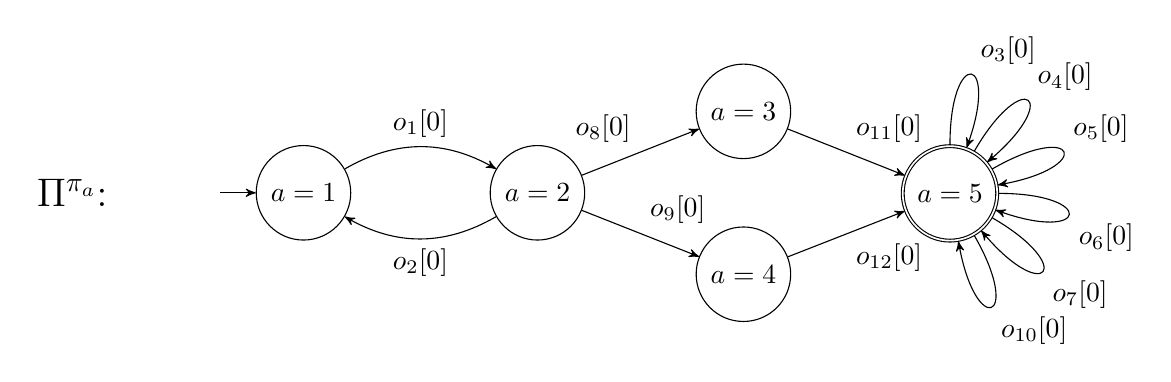
\begin{tikzpicture}[horizontal states, baseline]
        \node (label) {\Large $\Pi^{\pi_a}$:};
        \node[initial left, initial text=, state, right=of label] (s1) {$a=1$};
        \node[state, right=of s1] (s2) {$a=2$};
        \node[state, above right=of s2] (s3) {$a=3$};
        \node[state, below right=of s2] (s4) {$a=4$};
        \node[state, accepting, below right=of s3] (s5) {$a=5$};

        \path
            (s1) edge[bend left] node {\shortedgelabel{o_1}{0}} (s2)
            (s2) edge[bend left] node {\shortedgelabel{o_2}{0}} (s1)
            (s2) edge[] node {\shortedgelabel{o_8}{0}} (s3)
            (s2) edge[] node {\shortedgelabel{o_9}{0}} (s4)
            (s3) edge[] node {\shortedgelabel{o_{11}}{0}} (s5)
            (s4) edge[] node[swap] {\shortedgelabel{o_{12}}{0}} (s5)
            (s5) edge[out=90, in=70, looseness=15] node {\shortedgelabel{o_3}{0}} (s5)
            (s5) edge[out=60, in=40, looseness=15] node {\shortedgelabel{o_4}{0}} (s5)
            (s5) edge[out=30, in=10, looseness=15] node {\shortedgelabel{o_5}{0}} (s5)
            (s5) edge[out=0, in=-20, looseness=15] node {\shortedgelabel{o_6}{0}} (s5)
            (s5) edge[out=-30, in=-50, looseness=15] node {\shortedgelabel{o_7}{0}} (s5)
            (s5) edge[out=-60, in=-80, looseness=15] node {\shortedgelabel{o_{10}}{0}} (s5)
        ;
    \end{tikzpicture}

    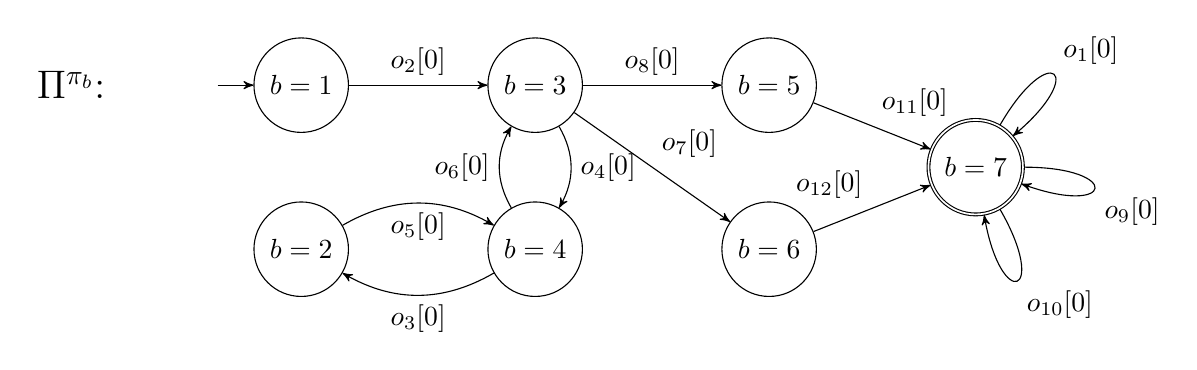
\begin{tikzpicture}[horizontal states, baseline]
        \node (label) {\Large $\Pi^{\pi_b}$:};
        \node[initial left, initial text=, state, right=of label] (s1) {$b=1$};
        \node[state, right=of s1] (s3) {$b=3$};
        \node[state, right=of s3] (s5) {$b=5$};
        \node[state, accepting, below right=of s5] (s7) {$b=7$};
        \node[state, below left=of s7] (s6) {$b=6$};
        \node[state, left=of s6] (s4) {$b=4$};
        \node[state, left=of s4] (s2) {$b=2$};

        \path
            (s1) edge[] node {\shortedgelabel{o_2}{0}} (s3)
            (s4) edge[bend left] node {\shortedgelabel{o_3}{0}} (s2)
            (s3) edge[bend left] node {\shortedgelabel{o_4}{0}} (s4)
            (s2) edge[bend left] node[swap] {\shortedgelabel{o_5}{0}} (s4)
            (s4) edge[bend left] node {\shortedgelabel{o_6}{0}} (s3)
            (s3) edge[] node {\shortedgelabel{o_7}{0}} (s6)
            (s3) edge[] node {\shortedgelabel{o_8}{0}} (s5)
            (s5) edge[] node {\shortedgelabel{o_{11}}{0}} (s7)
            (s6) edge[] node {\shortedgelabel{o_{12}}{0}} (s7)
            (s7) edge[out=60, in=40, looseness=15] node {\shortedgelabel{o_1}{0}} (s7)
            (s7) edge[out=0, in=-20, looseness=15] node {\shortedgelabel{o_9}{0}} (s7)
            (s7) edge[out=-60, in=-80, looseness=15] node {\shortedgelabel{o_{10}}{0}} (s7)
        ;
    \end{tikzpicture}

    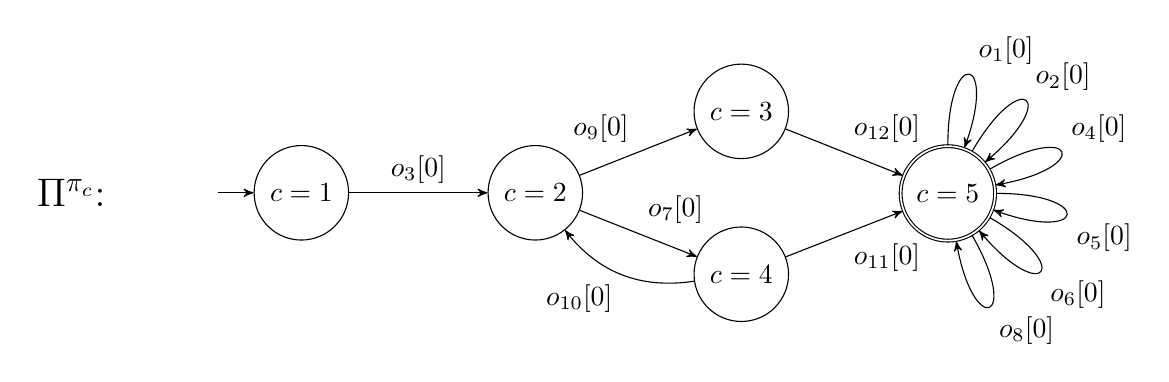
\begin{tikzpicture}[horizontal states, baseline]
        \node (label) {\Large $\Pi^{\pi_c}$:};
        \node[initial left, initial text=, state, right=of label] (s1) {$c=1$};
        \node[state, right=of s1] (s2) {$c=2$};
        \node[state, above right=of s2] (s3) {$c=3$};
        \node[state, below right=of s2] (s4) {$c=4$};
        \node[state, accepting, below right=of s3] (s5) {$c=5$};

        \path
            (s1) edge[] node {\shortedgelabel{o_3}{0}} (s2)
            (s2) edge[] node {\shortedgelabel{o_7}{0}} (s4)
            (s2) edge[] node {\shortedgelabel{o_9}{0}} (s3)
            (s4) edge[bend left] node {\shortedgelabel{o_{10}}{0}} (s2)
            (s4) edge[] node[swap] {\shortedgelabel{o_{11}}{0}} (s5)
            (s3) edge[] node {\shortedgelabel{o_{12}}{0}} (s5)
            (s5) edge[out=90, in=70, looseness=15] node {\shortedgelabel{o_1}{0}} (s5)
            (s5) edge[out=60, in=40, looseness=15] node {\shortedgelabel{o_2}{0}} (s5)
            (s5) edge[out=30, in=10, looseness=15] node {\shortedgelabel{o_4}{0}} (s5)
            (s5) edge[out=0, in=-20, looseness=15] node {\shortedgelabel{o_5}{0}} (s5)
            (s5) edge[out=-30, in=-50, looseness=15] node {\shortedgelabel{o_6}{0}} (s5)
            (s5) edge[out=-60, in=-80, looseness=15] node {\shortedgelabel{o_8}{0}} (s5)
        ;
    \end{tikzpicture}
    \end{center}
\end{document}
